\documentclass[a4paper, 11pt]{article}

\usepackage[utf8]{inputenc} % allow utf-8 input
\usepackage[T1]{fontenc}    % use 8-bit T1 fonts
\usepackage{hyperref}       % hyperlinks
\usepackage{url}            % simple URL typesetting
\usepackage{booktabs}       % professional-quality tables
\usepackage{amsfonts}       % blackboard math symbols
\usepackage{nicefrac}       % compact symbols for 1/2, etc.
\usepackage{microtype}      % microtypography
\usepackage[normalem]{ulem}
\usepackage{graphicx}

\title{From Word to Financial Time Series Embedding}

\author{
  Maxime De Bruyn \\
  Degroof Petercam Asset Management \\
  \texttt{m.debruyn@degroofpetercam.com} \\
  %% examples of more authors
  %% \And
  %% Coauthor \\
  %% Affiliation \\
  %% Address \\
  %% \texttt{email} \\
  %% \AND
  %% Coauthor \\
  %% Affiliation \\
  %% Address \\
  %% \texttt{email} \\
  %% \And
  %% Coauthor \\
  %% Affiliation \\
  %% Address \\
  %% \texttt{email} \\
  %% \And
  %% Coauthor \\
  %% Affiliation \\
  %% Address \\
  %% \texttt{email} \\
}

\begin{document}

\maketitle

\begin{abstract}
Pre-trained word vectors contributed to state of the art results in many Natural Language Processing tasks. In this work we show that the same algorithms can be applied to the embedding of financial time series.
Pre-trained vectors for financial time series are useful for visualizing an investable universe, embedding a portfolio of financial instruments, and can be used as context vectors in larger NLP networks. 
\end{abstract}

\section{Introduction}

Pre-trained word embeddings played a significant role in the advent of NLP with deep learning. The shift from shallow models based on very high dimensional data to dense vector representation helped achieve superior results on many NLP tasks. It sparked new state-of-the-art results in Neural Machine Translation, Sentence Classification or Question Answering \cite{DBLP:journals/corr/abs-1708-02709}. The same unsupervised training techniques can be applied to the embedding of financial time series (stocks, bonds, etc.), potentially leading to new breakthroughs in the field. 

Embedding financial time series is useful in three ways. First, an investor can visually explore his investable universe with dimensionality reduction techniques such as t-SNE. Second, drawing from the NLP field where sentences are represented as bag-of-words, portfolios of financial instruments can be represented as weighted bag-of-instruments. Third, pre-trained vectors can be used in larger NLP networks (for example predicting the impact of news on portfolios). More specifically, they can be used as context vectors in attentional layers.

In this work, two common word embedding techniques will be applied to the embedding of financial time series. Only minor changes are required to make them applicable to time series embedding.

\section{Models}

The goal of word embedding models is to learn a mapping from a list of words (a dictionary) to a vector space \(\mathbb{R}^d\). In practice, it is achieved by assigning each row of a matrix \(W^{n,d}\) to a word, where \(n\) is the number of words in the dictionary and \(d\) is the dimension of the word vectors. \(W^{1,d}\) represents the first word in the dictionary, \(W^{2,d}\) represents the second, etc.

The main idea behind the unsupervised word embedding approaches is that one would like the embedding vectors of similar words to have similar vectors. The current approach derives from the distributional hypothesis, stating that words are similar if they appear in similar contexts. In most cases, the contexts of a word are taken to be other words that appear around a focus word (defined by a sliding window of 2k+1 words) \cite{DBLP:journals/corr/Goldberg15c}. The similarity of two vectors can be measured by the dot product or the cosine similarity.
\begin{center}
the \dotuline{quick} \dotuline{brown} \underline{fox} \dotuline{jumps} \dotuline{over} the lazy dog
\end{center}
The words \dotuline{quick}, \dotuline{brown}, \dotuline{jumps} and \dotuline{over} are context words for the center word \underline{fox}.

Word embedding models use a large corpus of sentences to learn semantically related word vectors. In the context of financial markets, daily returns of financial instruments will be used as corpus.

Common unsupervised word-embedding algorithms include word2vec, GloVe and the Collobert and Weston algorithm. This work will apply the word2vec and GloVe algorithm to financial time series embedding. 

\subsection{Word2Vec}
The word2vec skip-gram algorithm \cite{DBLP:journals/corr/MikolovSCCD13}, learns a distributed representations of words in a vector space from a large amount of unstructured text data. The training objective of the skip-gram model is to find word representations that are useful for predicting the surrounding words in a sentence or a document. More formally, given a sequence of training words \(w_1\), \(w_2\), \(w_3\), …, \(w_T\), the objective of the skip-gram model is to maximize the average log probability
\begin{equation}
\frac{1}{T}\sum_{t=1}^{T}\sum_{-c\leq j\leq c,j\neq 0} \log{p(w_{t+j}\mid w_t)}
\end{equation}
where \(c\) is the size of the training context. The basic skip-gram model defines \(p(w_{t+j}\mid w_t)\) using the softmax function:
\begin{equation}
p(w_O \mid w_I) = \frac{\exp(v_{w_O}'{ }^\top v_{w_I})}{\sum_{w=1}^{W} \exp(v_{w}'{ }^\top v_{w_I})}
\end{equation}
where \(v_w\) and \(v_w^{'}\) are the input and output vector representations of \(w\). and \(W\) is the number of words in the vocabulary. As the number of instruments in our universe is limited we can stick to the simple skip-gram model. The interested reader is invited to read the negative sampling variant \cite{DBLP:journals/corr/MikolovSCCD13}.

The intuition behind this model is to train a set of vectors such that when two words appear in the same context window, the dot product of their vector \(v_{w_O}'{ }^\top v_{w_I}\) is high. Similarly, if two words do not appear in the same context, their dot product \(v_{w}'{ }^\top v_{w_I}\) should be low.

The reasoning that similar words appear in the same context can be extended to financial markets. Similar instruments will tend to trade similarly in any given day. The context window becomes a function that ranks instruments according to their relative absolute performance on a given day. Instead of sentences, we use trading days.

\begin{table}[htb]
\begin{center}
\begin{tabular}{|c|c|c|c|c|c|c|}
  \hline
  NVDA & AAPL & MSFT & CSCO & SNAP & FB & GOOG \\
  \hline
  -2\% & -0.2\% & -0.7\% & +0.2\% & +0.5\% & +1.2\% & +2\% \\
  \hline
\end{tabular}
\end{center}
\caption{Simulated daily return for 6 stocks}
\label{table:dailyperf}
\end{table}
According to table \ref{table:dailyperf}, on that day with a context window of size 2, the context for CSCO (+0.2\%) is AAPL (-0.2\%) and SNAP (+0.5\%), because their performance are the closest to the performance of SNAP.

\subsection{GloVe}

The GloVe (Global Vectors \cite{pennington2014glove}) algorithm has the same goal as word2vec: learning good word vectors representation. They differ in their implementation and measure of similarity. While the word2vec algorithm uses raw sentences and context windows to measure the similarity between words, the GloVe algorithm will use corpus statistics as a measure of similarity between words.

The training objective of the GloVe algorithm is to learn word vectors so that their dot products equals the logarithm of the words' probability of co-occurrence. The co-occurrence matrix measures the number of times the word \(j\) occurs in the context (defined by a context window length) of word \(i\). Formally, the training objective is the least squared regression model:
\begin{equation}
J = \sum_{i,j=1}^{V} f(X_{ij})(w_i^T \tilde{w}_j + b_i + \tilde{b}_j - \log X_{ij})^2
\end{equation}
where \(V\) is the size of the vocabulary, \(f(X_{ij})\) is a weighting function, \(w_i\) is the word vector associated to \(i\) in matrix \(W\), \(b_i\) is a bias term associated with word \(i\) and \(X_{ij}\) is the co-occurrence probability. The authors choose to have two different word vector matrices: one for the input words \(X\) and one for the output words \(\tilde{X}\).

The GloVe algorithm can be transformed to fit time series embedding by switching the co-occurrence matrix with the correlation or covariance matrix.  

\paragraph{Covariance}
The training objective is now to learn entity vectors so that their dot product equals their pairwise covariance.
\begin{equation}
J = \sum_{i,j=1}^{V} (v_i^T v_j - X_{ij})^2
\end{equation}
where \(V\) is the number of security under analysis, \(v_i\) is the vector associated to instrument \(i\), and \(X_{ij}\) is the covariance between the security \(i\) and \(j\).

\paragraph{Correlation}
The training objective is now to learn entity vectors so that their cosine similarity equals their pairwise correlation or covariance.
As the correlation of an entity with itself is one, cosine similarity is a better choice than dot product.
\begin{equation}
J = \sum_{i,j=1}^{V} (\frac{v_i^T v_j }{\left \| v_i \right \|\left \| v_j \right \|} - X_{ij})^2
\end{equation}
where \(V\) is the number of security under analysis, \(v_i\) is the vector associated with instrument \(i\), and \(X_{ij}\) is the correlation between the security \(i\) and \(j\).



\section{Data}
The investable universe is defined by the holdings of the Vanguard Total World Stock ETF as of the 29\textsuperscript{th} of December 2017. It holds a total of 7857 instruments from 11 sectors, 24 industry groups, 37 currencies and 69 countries.

Time series are constructed by downloading the total return index for each constituent from the 31\textsuperscript{st} of December 2016 to the 31\textsuperscript{st} of December 2017. From these prices,  the daily returns and correlation matrix are computed. Instruments with little trading history were discarded.

The code and resulting trained vectors are available on Github\footnote{\url{https://github.com/maximedb/stock2vec}}.

\section{Results and Analysis}
The three models (Glove Covariance, Glove Correlation and Skip-Gram) were trained using Pytorch \cite{paszke2017automatic}. The dimension of trained vectors is 300. The optimizer used is the Adam algorithm \cite{DBLP:journals/corr/KingmaB14}. The parameters are detailed in the table \ref{table:models}
\begin{table}[htb]
\begin{center}
\begin{tabular}{|c|c|c|c|c|c|c|}
  \hline
  Model & Learning rate & Batch size & Epoch & Loss\\
  \hline
  GloveCov & 0.0005 & 2500 & 20 & 3.16e-6\\
  GloveCor & 0.0005 & 2500 & 20 & 0.0096\\
  Skip-Gram & 0.0005 & 2500 & 30 & 7.5893\\
  \hline
\end{tabular}
\end{center}
\caption{Models specifications}
\label{table:models}
\end{table}

The quality of word embeddings is often evaluated on analogical reasoning tasks introduced by \cite{DBLP:journals/corr/abs-1301-3781}. The tasks consists of finding the missing word in analogical reasoning exercise. Given the words "Germany" and "Berlin", can the model guess what follows after "France" ? A good model needs to guess "Paris". In practice, this is implemented using the difference of vectors. If we do \(vec("Berlin") - vec("Germany") + vec("France")\), the resulting vector should be close to \(vec("Paris")\). There exists no such dataset for analogical reasoning about financial time series. We will evaluate the quality of the learned vectors in other ways.

\subsection{Visual Exploration}
The first way to assess the quality of vectors is to inspect them visually. Pre-trained vectors of high dimensional space can be visually analyzed with PCA or t-SNE. Both method are dimensionality reduction technique. An interactive visualization is available on this \href{https://projector.tensorflow.org/?config=https://raw.githubusercontent.com/maximedb/stock2vec/master/embeddings/config.json}{link}\footnote{\url{https://projector.tensorflow.org/?config=https://raw.githubusercontent.com/maximedb/stock2vec/master/embeddings/config.json}}.

\begin{figure}[h]
\centering
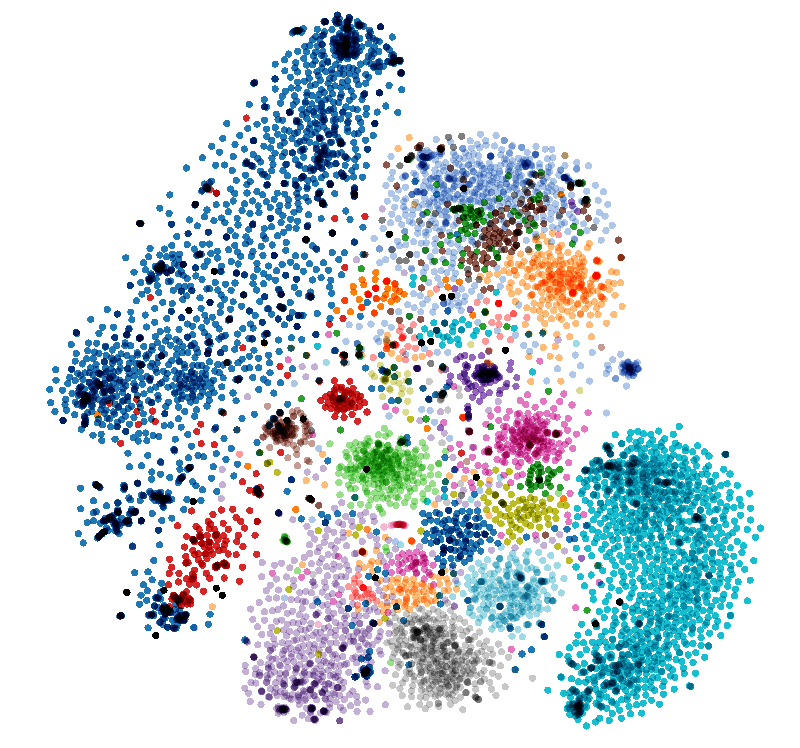
\includegraphics[scale=0.33]{tsne_glove_cov.PNG}
\caption{T-SNE representation of the GloVe Covariance vectors (colored by currency). JPY instruments are clustered on the bottom right (green), USD instruments are clustered on the top left, European currencies (EUR, SEK, GBP, etc.) are clustered on the top right.}
\end{figure}

\subsection{Correlation and covariance approximation}
A second way to assess the quality of the trained vectors is to analyze how closely they relate to the true correlation and covariance matrix. The learned correlation matrix can be estimated by computing the cosine similarity between the vectors. The covariance matrix can be estimated by computing the dot product between the vectors (only applicable to the GloveCov model). The resulting matrices are then compared against the true matrix and the mean absolute difference is reported. The reader should bear in mind that GloVe algorithms were trained to predict the covariance or correlation between instruments, so the comparison is unfair for the skip-gram algorithm.

\begin{table}[h]
\begin{center}
\begin{tabular}{|c|c|c|c|c|c|c|}
  \hline
  Model & Correlation & Covariance \\
  \hline
  GloveCov & 0.004 (0.012) & 1.105e-06 (3.721e-06)\\
  GloveCor & 0.002 (0.010) & -\\
  Skip-Gram & 0.085 (0.069) & -\\
  \hline
\end{tabular}
\end{center}
\caption{Mean absolute difference between the true matrix and the estimated matrix}
\label{table:correstimation}
\end{table}
Although the GloveCov algorithm was trained to predict the covariance between two instruments, it can also predict the correlation between these instruments with a reasonable accuracy.


\subsection{Bag-of-instruments}
A third way to assess the quality of word vectors is to check whether vectors can be aggregated and convey information at the level of the portfolio. To do this, 11 sector portfolios were created along with their true correlation and covariance matrix. Each sector was also attributed a bag-of-instruments according to the formula number (\ref{equation:bagofsec}).

A Bag-of-instruments is a weighted average of its constituents' vectors.
\begin{equation}
\sum_{i\, \epsilon \, P} w_iv_i
\label{equation:bagofsec}
\end{equation}
where \(P\) is the portfolio containing a set of stocks, \(w_i\) is the weight of stock \(i\) in the portfolio, and \(v_i\) is the vector associated to stock \(i\).

\begin{table}[htb]
\begin{center}
\begin{tabular}{|c|c|c|c|c|c|c|}
  \hline
  Model & Correlation & Covariance \\
  \hline
  GloveCov & 0.003 (0.003) & 1.054e-7 (1.849e-7)\\
  GloveCor & 0.021 (0.017) & -\\
  Skip-Gram & 0.206 (0.158) & -\\
  \hline
\end{tabular}
\end{center}
\caption{Mean absolute difference between the true matrix and the estimated matrix}
\label{table:bagofstocks}
\end{table}

Table \ref{table:bagofstocks} summarizes the result of the comparison between the estimated correlation and covariance matrices relative to the true correlation and covariance matrices.
The GloveCov model did not loose information in the process. Its prediction power stayed the same (or improved a little bit). The GloveCor model lost prediction power by a factor of 10. The skip-gram model is completely wrong.   


\section{Future Work}
Weighted bag-of-instruments can be extended to cross-sectional factor embedding, which can be useful for quickly assessing a portfolio exposure to such factors. One can rank the universe according to a factor (price-to-book value for example), and make a weighted bag-of-instruments for each quintile. The factor embedding is equal to the first quintile bag-of-instruments minus the last one. A portfolio exposition to this factor is the cosine similarity between the portfolio embedding and the factor embedding.

Not all entries in the covariance and correlation matrix were computed using the same amount of information (some trading histories can be smaller than others). The GloVe algorithm can be tweaked to take into account the number of days used in the calculation of the covariance. The original GloVe algorithm used a weighting factor, it could be transformed to fit this goal.

The skip-gram with negative sampling can be more suited to the goal of financial time series embedding as it can have a sense of similarity and dissimilarity with the use of negative examples.

The two proposed algorithms (Skip-Gram and Glove) are unable to embed previously unseen words. The same applies to the embedding of financial time series. If a company is about to IPO, it has no trading history. Fasttext \cite{bojanowski2016enriching} solved this issue by treating each word as the sum of its part (n-gram). This can also be used in the context of financial markets. 


\section{Conclusion}
As a conclustion, it is possible to tweak common word embedding techniques for the embedding of financial time series. Pre-trained vectors can be learned either via the skip-gram or the GloVe algorithm. The GloVe model with the covariance method is preferred over the other algorithms as its loss function is directly interpretable and it showed better results on the bag-of-instruments analysis. 

The embedding of financial time series can be useful for the visual exploration of the investable universe. Furthermore, individual instrument vectors can be combined to embed entire portfolios or indexes via bag-of-instruments, a linear combination of instruments' vectors.

Even though some areas remain to explore, it is encouraging to see that financial time series can be embedded into vectors. These vectors can then be used in other contexts, such as Natural Language Processing.


\bibliographystyle{plain} 
\bibliography{refs} % Entries are in the "refs.bib" file

\end{document}
